\documentclass[12pt,a4paper]{article}

\usepackage[spanish,es-nodecimaldot]{babel}
\usepackage[utf8]{inputenc}
\usepackage[T1]{fontenc}
\usepackage{lmodern}
\usepackage{geometry}
\usepackage{graphicx}
\usepackage{float}
\usepackage{hyperref}
\usepackage{booktabs}
\usepackage{array}
\usepackage{enumitem}
\usepackage{xcolor}
\usepackage{setspace}
\usepackage{caption}
\usepackage{listings}
\usepackage{xcolor}

\lstdefinestyle{pythonstyle}{
    language=Python,
    basicstyle=\ttfamily\small,
    numbers=left,
    numberstyle=\tiny,
    stepnumber=1,
    numbersep=8pt,
    showstringspaces=false,
    breaklines=true,
    breakatwhitespace=true,
    frame=single,
    tabsize=4,
    captionpos=b,
    keywordstyle=\color{blue},
    commentstyle=\color{gray},
    stringstyle=\color{teal}
}

\geometry{margin=2.5cm}
\setstretch{1.15}
\hypersetup{
    colorlinks=true,
    linkcolor=black,
    urlcolor=blue,
    citecolor=black
}

\title{\textbf{Tarea 1: Herramientas de Visualización de Datos}\\
Tema: \textbf{LLMs}}
\author{
    Isaías Carte Figueroa \\
    Nicolás Gonzáles \\
    Benjamín Olguín Pozo
}
\date{Visualización de Datos -- Semestre I 2026}

\begin{document}

\maketitle
\thispagestyle{empty}

\begin{center}
Universidad Técnica Federico Santa María \\
Departamento de Informática
\end{center}

\vspace{1cm}

\section{Introducción}

Para esta primera tarea se seleccionó como tema central el estudio de los \textit{Large Language Models} (LLMs), debido a su rápido crecimiento, diversidad de aplicaciones y relevancia actual dentro del desarrollo de sistemas de inteligencia artificial. El objetivo del trabajo fue analizar este fenómeno desde tres dimensiones complementarias, no convencionales y coherentes.

En conjunto, el informe aborda los LLMs desde una perspectiva histórica, competitiva y de uso práctico. La primera dimensión estudia la evolución temporal de los modelos y la participación de las organizaciones desarrolladoras; la segunda analiza la relación entre rendimiento técnico y costo de inferencia; y la tercera se enfoca en la preferencia humana observada en enfrentamientos directos entre modelos. Esta combinación permite construir una visión más amplia del ecosistema actual de los LLMs.

\section{Metodología general}

Cada integrante seleccionó dos criterios de análisis distintos, recopiló datos desde fuentes específicas y desarrolló una visualización en Python procurando evitar gráficos tradicionales.

Las visualizaciones elegidas fueron las siguientes:

\begin{itemize}[leftmargin=1.2cm]
    \item \textit{Streamgraph} para representar la evolución temporal de modelos y la participación de organizaciones.
    \item Gráfico de \textit{Parallel Coordinates} para contrastar rendimiento por benchmark y costo de inferencia.
    \item Diagrama de \textit{Sankey} para representar victorias entre modelos según preferencia humana.
\end{itemize}

\section{Desarrollo individual}

\subsection{Evolución temporal y participación organizacional}

\subsubsection*{Criterios seleccionados}
Los criterios de análisis escogidos fueron los siguientes:

\begin{itemize}[leftmargin=1.2cm]
    \item \textbf{Evolución temporal de modelos LLM.}
    \item \textbf{Participación de organizaciones desarrolladoras.}
\end{itemize}

\subsubsection*{Justificación}
Estos criterios permiten analizar el desarrollo de los LLM desde una perspectiva histórica y competitiva. La evolución temporal permite observar en qué períodos aumenta la aparición de modelos relevantes, mientras que la participación por organización permite identificar qué empresas concentran mayor protagonismo en este proceso. Así, esta sección entrega una base contextual para comprender cómo se ha configurado el ecosistema actual de modelos de lenguaje.

\subsubsection*{Fuente de datos}
Se utilizaron datos extraídos desde la base de modelos notables de Epoch AI:

\begin{itemize}[leftmargin=1.2cm]
    \item \url{https://epoch.ai/data/ai-models?view=table&tab=notable}
\end{itemize}

\subsubsection*{Gráfico}
Se utilizó un \textbf{Streamgraph}, ya que este tipo de visualización permite representar la evolución temporal de distintas categorías manteniendo una lectura fluida de los cambios en el tiempo y del peso relativo de cada organización.

\begin{figure}[H]
    \centering
    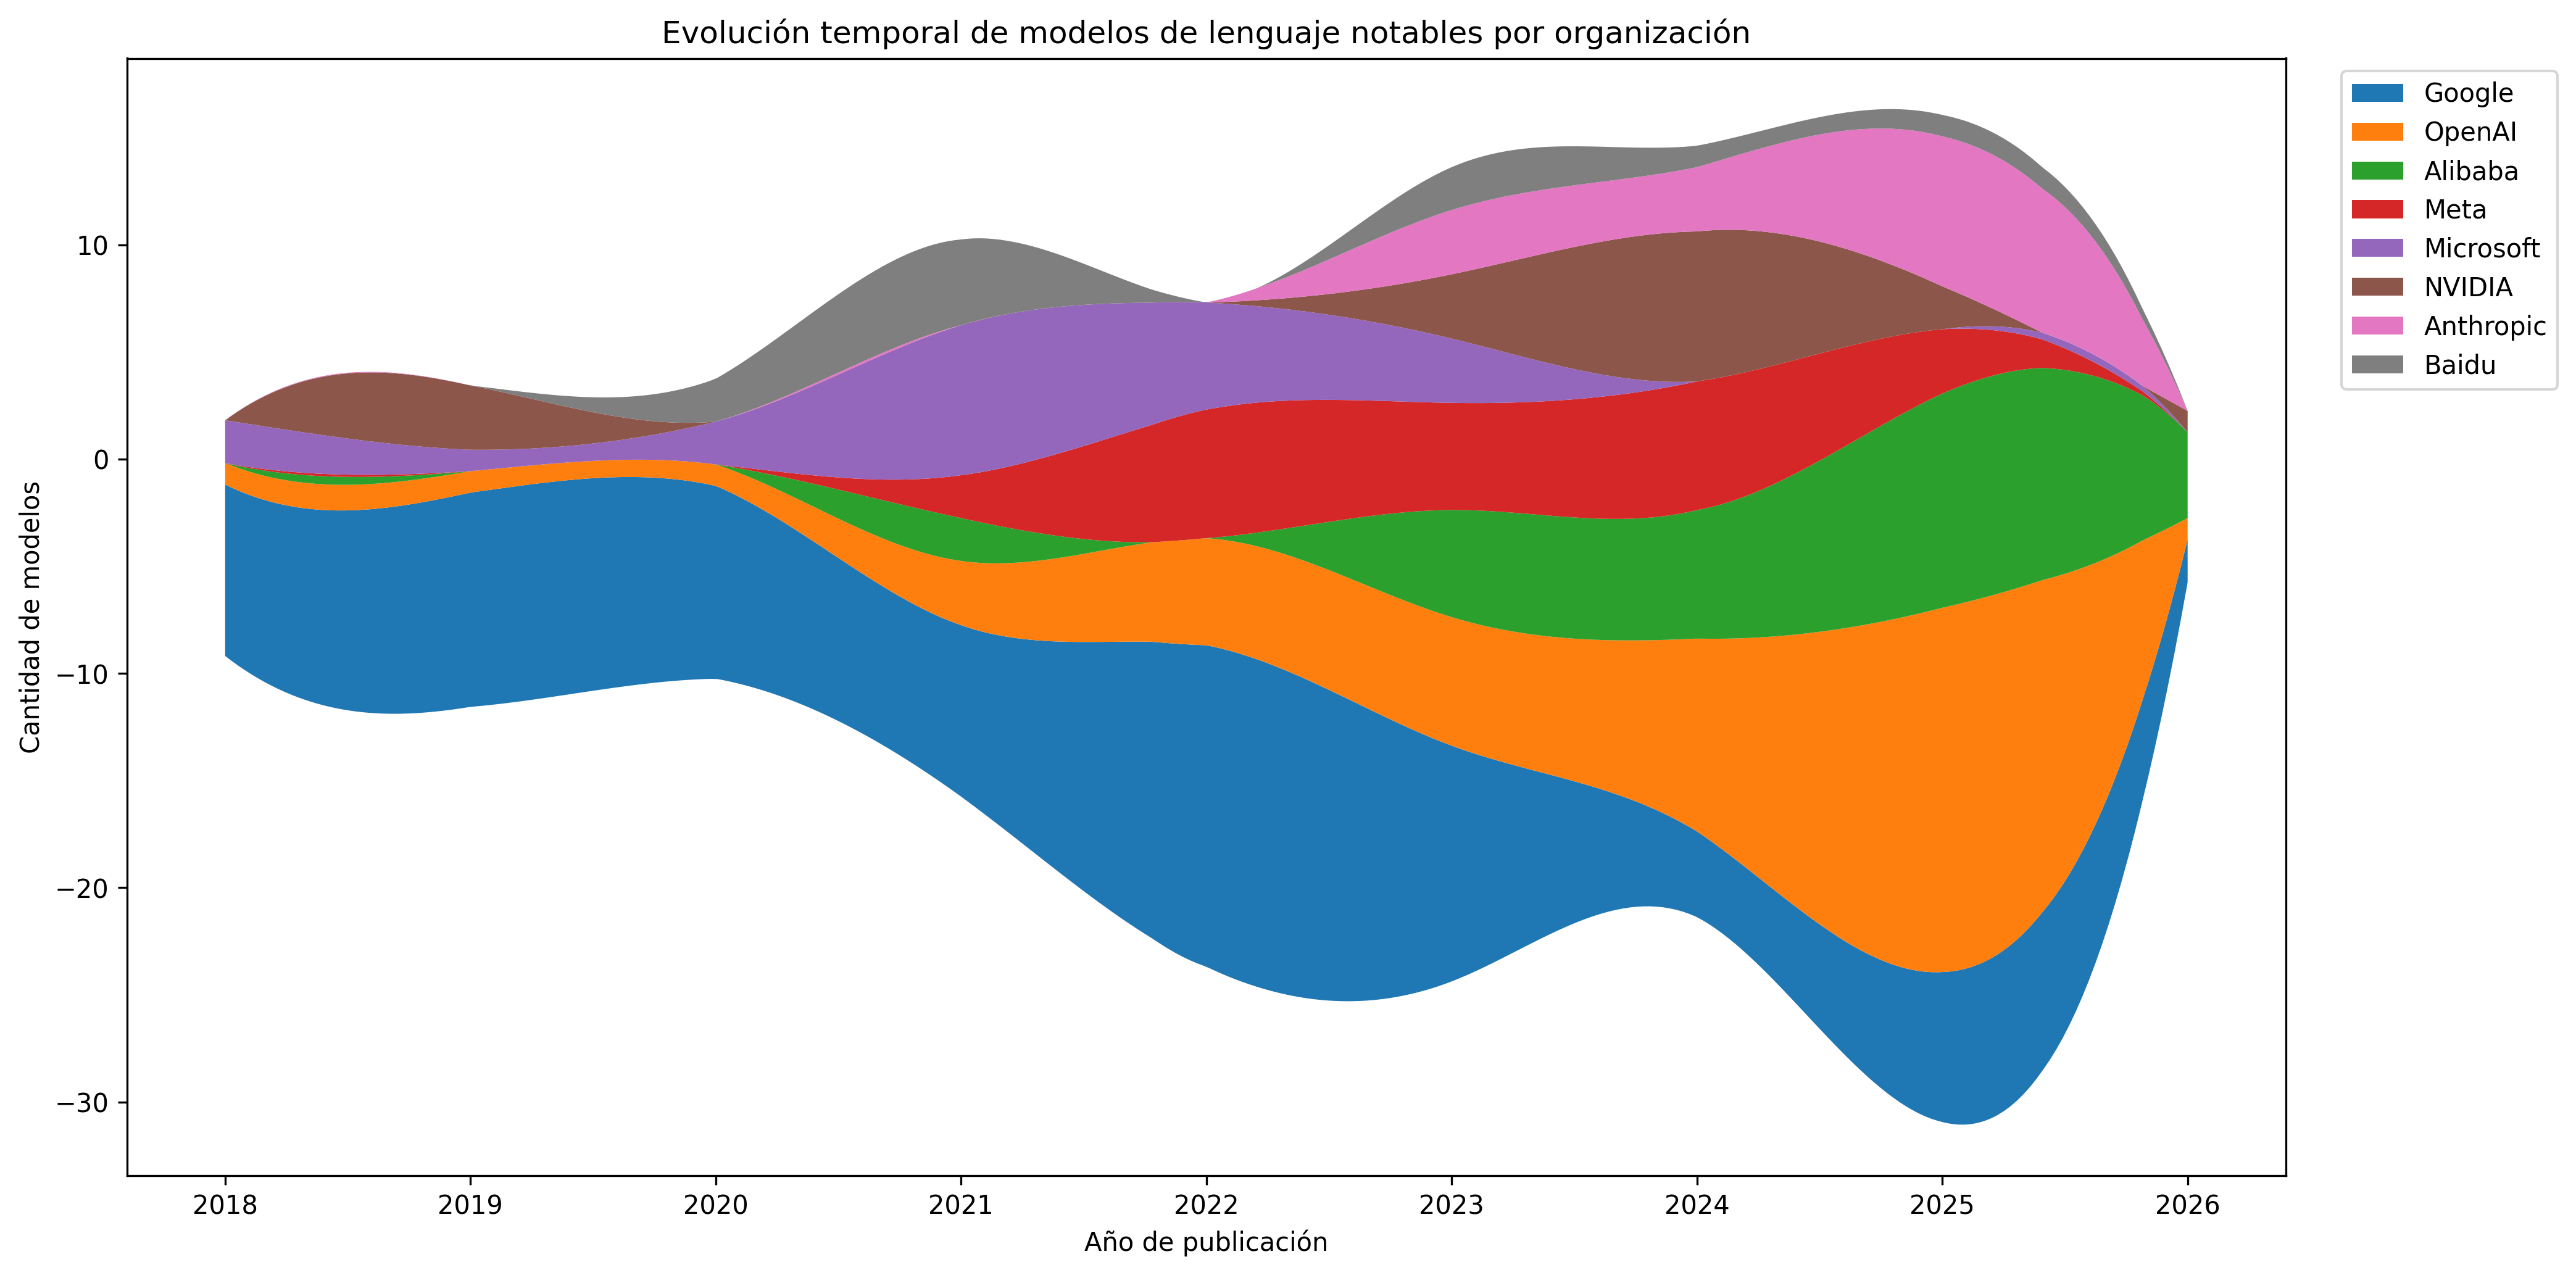
\includegraphics[width=0.95\textwidth]{Parte Isaias/streamgraph_suave.png}
    \caption{Evolución temporal de modelos LLM y participación de organizaciones desarrolladoras.}
    \label{fig:streamgraph-isaias}
\end{figure}

\subsubsection*{Conclusiones}
Entre 2018 y 2025 se observa un aumento sostenido en la aparición de modelos de lenguaje notables, lo que sugiere una aceleración importante en el desarrollo de los LLMs durante los últimos años. A su vez, Google y OpenAI destacan como las organizaciones con mayor peso relativo en el gráfico, aunque otras como Anthropic, Meta y Microsoft también incrementan su presencia en el período más reciente.

En consecuencia, la visualización sugiere que el desarrollo de los LLMs no ha sido uniforme a lo largo del tiempo, sino que se concentra especialmente desde 2022 en adelante, etapa en la que más organizaciones comienzan a competir de forma visible.

\subsection{Rendimiento por benchmark y costo de inferencia}

\subsubsection*{Criterios seleccionados}
Los criterios definidos para esta parte fueron:

\begin{itemize}[leftmargin=1.2cm]
    \item \textbf{Rendimiento por dominio}, medido mediante benchmarks estandarizados.
    \item \textbf{Costo de inferencia}, expresado en dólares por millón de tokens.
\end{itemize}

Los benchmarks considerados fueron:

\begin{itemize}[leftmargin=1.2cm]
    \item \textbf{MATH:} preguntas matemáticas.
    \item \textbf{GPQA:} preguntas científicas a nivel de PhD.
    \item \textbf{MMLU:} preguntas y tareas de conocimiento general.
    \item \textbf{HumanEval:} generación de código a partir de lenguaje natural.
\end{itemize}

\subsubsection*{Justificación}
Estos criterios permiten evaluar los LLMs desde una perspectiva de viabilidad práctica y comercial, más allá del avance técnico aislado. El rendimiento por sí solo no siempre basta para decidir qué modelo implementar en un entorno real; al cruzarlo con el costo de inferencia es posible estimar con mayor claridad la conveniencia de uso de cada alternativa.

\subsubsection*{Fuente de datos}
Los datos fueron recopilados desde las siguientes fuentes:

\begin{itemize}[leftmargin=1.2cm]
    \item \url{https://artificialanalysis.ai}
    \item \url{https://huggingface.co/spaces/open-llm-leaderboard/open_llm_leaderboard#/}
\end{itemize}

\subsubsection*{Gráfico}
Se utilizó un \textbf{gráfico de coordenadas paralelas} (\textit{Parallel Coordinates Plot}), adecuado para comparar múltiples variables cuantitativas de manera simultánea y visualizar perfiles de desempeño de distintos modelos.

\begin{figure}[H]
    \centering
    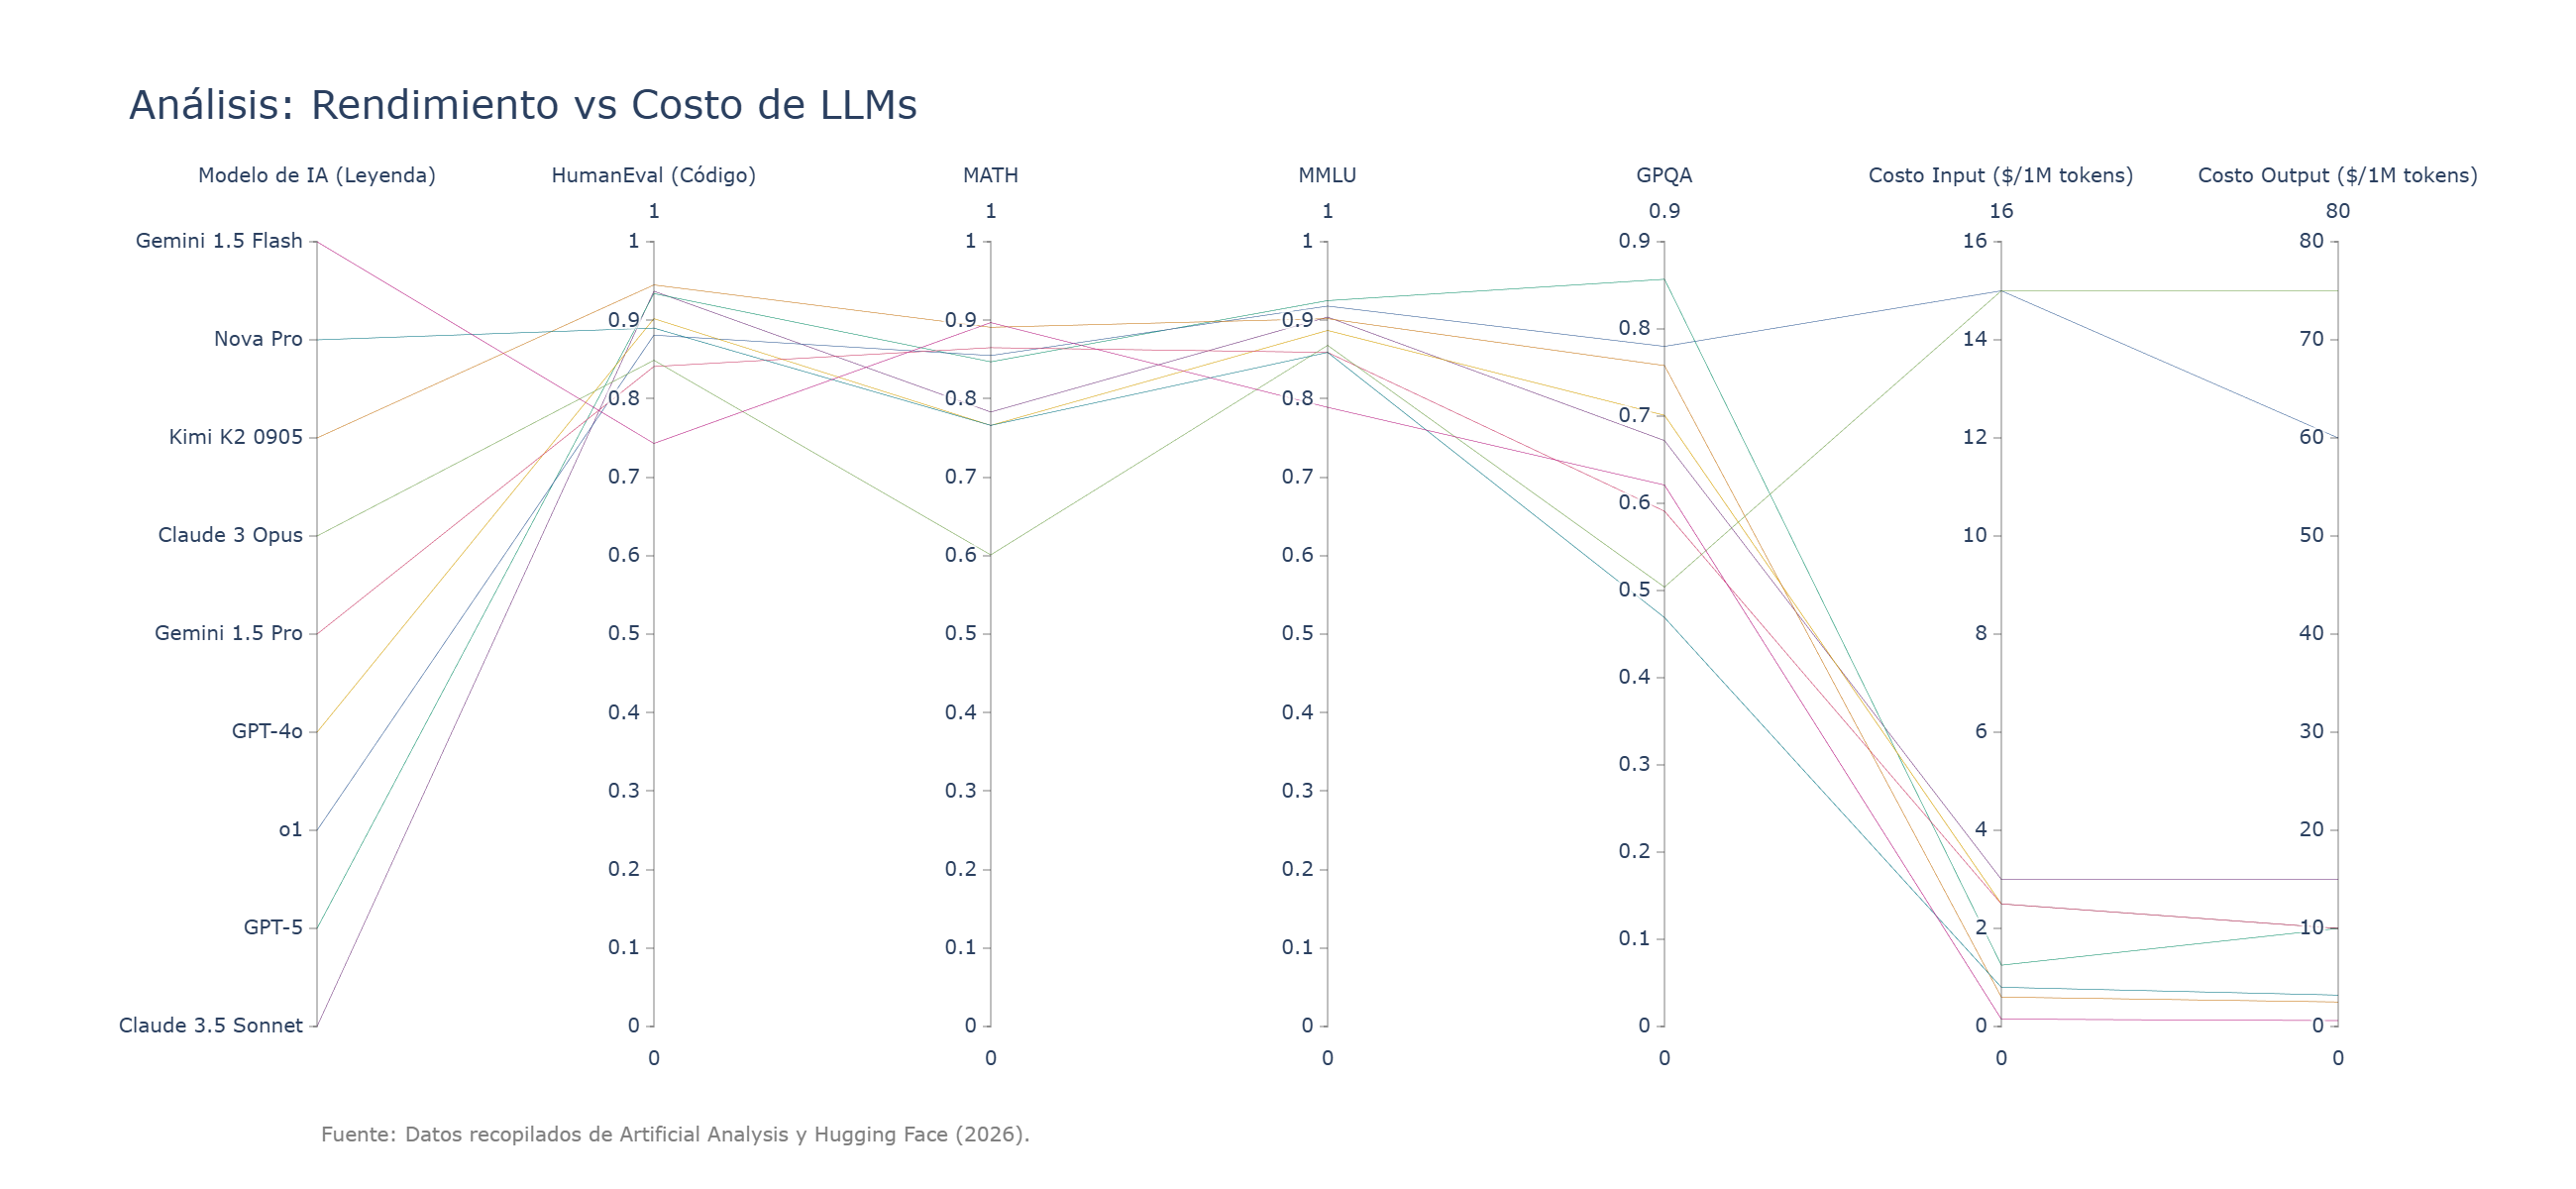
\includegraphics[width=0.95\textwidth]{Parte Nicolas/coordenadas_paralelas.png}
    \caption{Comparación entre rendimiento por benchmark y costo de inferencia de distintos LLMs.}
    \label{fig:parallel-nicolas}
\end{figure}

\subsubsection*{Conclusiones}
El gráfico permite observar que no existe una relación estrictamente lineal entre precio y rendimiento general. Algunos modelos con costos altos no dominan todas las dimensiones técnicas, mientras que ciertos modelos más económicos muestran resultados competitivos en métricas específicas.

Por otra parte, también se aprecia que alcanzar rendimientos sobresalientes en tareas de razonamiento experto o programación compleja suele seguir asociado a modelos de gama alta. Esto sugiere una segmentación del mercado, donde el costo adicional puede justificarse dependiendo del tipo de tarea que se desea resolver.

\subsection{Preferencia humana y competencia directa entre modelos}

\subsubsection*{Criterios seleccionados}
Los criterios definidos para esta sección fueron:

\begin{itemize}[leftmargin=1.2cm]
    \item \textbf{Desempeño relativo de los LLM según preferencia humana.}
    \item \textbf{Estructura de competencia entre modelos en enfrentamientos directos.}
\end{itemize}

El primer criterio busca medir qué tan bien se desempeña cada modelo cuando compite contra otros en comparaciones reales. El segundo permite analizar no solo qué modelos ganan más, sino también frente a qué rivales obtienen esas victorias.

\subsubsection*{Justificación}
Estos criterios permiten estudiar a los LLM desde una dimensión diferente al rendimiento técnico tradicional, enfocándose en comparaciones directas evaluadas por personas. De este modo, el análisis se acerca más a situaciones de uso práctico, donde importa no solo el benchmark, sino también cuál modelo resulta preferido en interacciones reales.

\subsubsection*{Fuente de datos}
Para esta sección se utilizó el siguiente dataset:

\begin{itemize}[leftmargin=1.2cm]
    \item \texttt{lmarena-ai/arena-human-preference-55k}
    \item \url{https://huggingface.co/datasets/lmarena-ai/arena-human-preference-55k}
\end{itemize}

\subsubsection*{Gráfico}
Se utilizó un \textbf{diagrama de Sankey}, ya que este tipo de visualización permite representar flujos de victorias entre modelos, conectando ganadores con derrotados y mostrando con el grosor de cada vínculo la frecuencia de dichos resultados.

\begin{figure}[H]
    \centering
    % Reemplazar por la ruta definitiva de la imagen exportada
    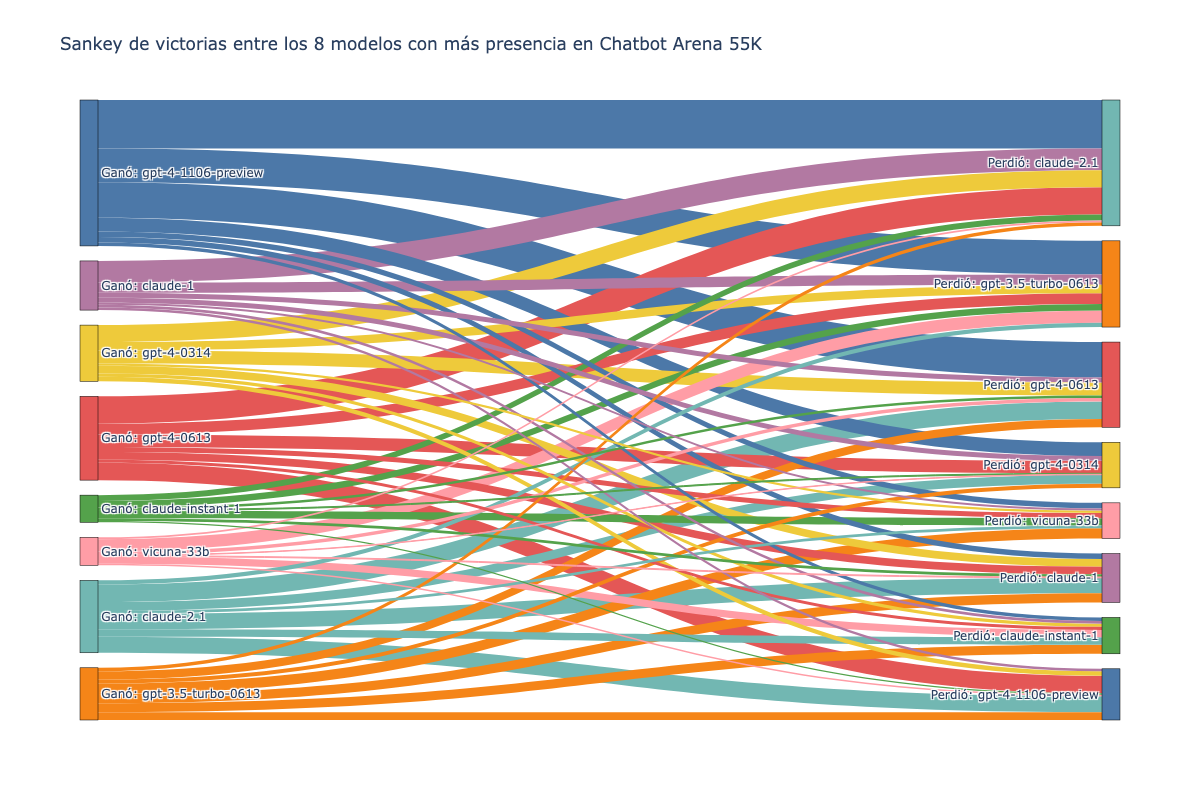
\includegraphics[width=0.95\textwidth]{Parte Benjamin/sandkey.png}
    \caption{Flujo de victorias entre modelos con mayor presencia en Chatbot Arena.}
    \label{fig:sankey}
\end{figure}

\subsubsection*{Conclusiones}
La visualización muestra que la preferencia humana no se distribuye de manera homogénea entre los modelos analizados. Algunos modelos concentran una mayor cantidad de victorias, mientras que otros acumulan más derrotas, lo que sugiere diferencias claras de desempeño relativo en enfrentamientos directos.

Además, se aprecia una estructura competitiva jerárquica: ciertos modelos derrotan repetidamente a varios rivales, mientras otros aparecen más frecuentemente en la posición de derrota. En conjunto, esto indica que la evaluación humana permite distinguir patrones de dominancia y competencia dentro del ecosistema de LLMs.

\section{Trabajo grupal con IA generativa}

\subsection{Objetivo}
Como complemento a las visualizaciones individuales, se incorporó una cuarta visualización generada con apoyo de una herramienta de IA generativa. Esta visualización tuvo como propósito integrar una perspectiva comparativa adicional sobre el ecosistema de los LLMs.

\subsection{Prompt utilizado}
Genera en Python un bump chart usando el dataset de modelos notables de Epoch AI. Filtra modelos de lenguaje entre 2018 y 2025, agrupa organizaciones equivalentes como Google y DeepMind, calcula el ranking anual por cantidad de modelos y grafica la evolución de las principales organizaciones.
\begin{quote}
\end{quote}

\subsection{Código generado}
\lstinputlisting[
    style=pythonstyle,
    caption={Código fuente del archivo utilizado para generar la visualización grupal del ranking anual de organizaciones por cantidad de modelos LLM notables.},
    label={lst:bumpchart_llm_orgs}
]{bumpchart_llm_orgs.py}
\begin{verbatim}
\end{verbatim}

\subsection{Visualización final}
% Reemplazar por la ruta final de la cuarta visualización
\begin{figure}[H]
    \centering
    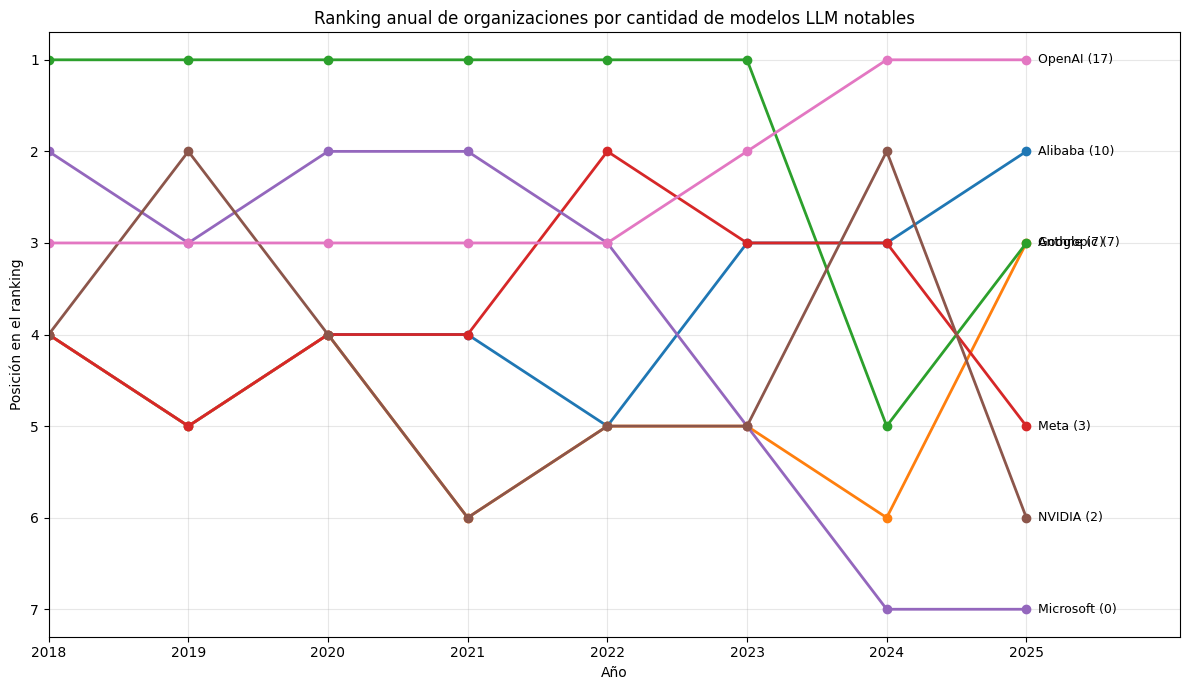
\includegraphics[width=0.95\textwidth]{bumpchart.png}
    \caption{Visualización grupal generada con apoyo de IA generativa.}
    \label{fig:bumpchart}
\end{figure}

\subsection{Conclusión grupal}
Considerando las tres visualizaciones individuales y la visualización grupal, se observa que el fenómeno de los LLMs puede abordarse desde múltiples dimensiones complementarias. La evolución histórica muestra una aceleración reciente en el desarrollo del área; la comparación entre costo y rendimiento expone tensiones entre capacidad técnica y viabilidad de implementación; y la preferencia humana revela que el desempeño percibido en enfrentamientos reales no siempre coincide de manera exacta con la lógica de los benchmarks.

En conjunto, el trabajo sugiere que el análisis de los LLMs requiere una mirada multidimensional. No basta con estudiar cuándo aparecieron los modelos, cuánto rinden o cuánto cuestan, sino también cómo son valorados por las personas y cómo se posicionan dentro de una red competitiva más amplia.

\section{Fuentes de datos}

\begin{itemize}[leftmargin=1.2cm]
    \item Epoch AI: \url{https://epoch.ai/data/ai-models?view=table&tab=notable}
    \item Artificial Analysis: \url{https://artificialanalysis.ai}
    \item Hugging Face Open LLM Leaderboard:\\
    \url{https://huggingface.co/spaces/open-llm-leaderboard/open_llm_leaderboard#/}
    \item Hugging Face Dataset: \\
    \url{https://huggingface.co/datasets/
    lmarena-ai/arena-human-preference-55k}
\end{itemize}

\section{Repositorio GitHub}

El código fuente, los datasets utilizados y los archivos asociados a esta tarea se encuentran disponibles en el siguiente repositorio:

\begin{center}
\url{https://github.com/IsaiasACF/Proyecto-Visualizacion-de-datos}
\end{center}

\section{Responsabilidad individual}

\begin{table}[H]
\centering
\begin{tabular}{>{\raggedright\arraybackslash}p{3cm} >{\raggedright\arraybackslash}p{10cm}}
\toprule
\textbf{Integrante} & \textbf{Aporte realizado} \\
\midrule
Isaias & Recolección de datos históricos desde Epoch AI, construcción del streamgraph y redacción de criterios, justificación y conclusiones asociadas a la evolución temporal y participación de organizaciones. \\
\addlinespace
Nicolás & Recolección de datos de benchmarks y costo de inferencia, construcción del gráfico de coordenadas paralelas y redacción de criterios, justificación y conclusiones asociadas a rendimiento técnico y costo. \\
\addlinespace
Benjamin & Selección del dataset de preferencias humanas, construcción del diagrama de Sankey y redacción de criterios, justificación y conclusiones sobre competencia directa y preferencia humana entre LLMs. \\
\bottomrule
\end{tabular}
\caption{Distribución de responsabilidades dentro del grupo.}
\label{tab:responsabilidad}
\end{table}

\end{document}